\documentclass[12pt,a4paper]{article}
\usepackage[utf8]{inputenc}
\usepackage[T1]{fontenc}
\usepackage{amsmath}
\usepackage{amsfonts}
\usepackage{amssymb}
\usepackage{graphicx}
\usepackage[indonesian]{babel}
\usepackage[left=2.00cm, right=2.00cm, top=2.00cm, bottom=2.00cm]{geometry}
\usepackage{float}
\usepackage{tikz}
\newcommand*\circled[1]{\tikz[baseline=(char.base)]{\node[shape=circle,draw,inner sep=2pt] (char) {#1};}}

\title{Jawaban Tugas 9 - Pengolahan Sinyal Digital\\
	Discreet Fourier Transform (DFT)}

% remove spacing around date:
\usepackage{titling}
\predate{}
\postdate{}
\date{}

\begin{document}
	\maketitle
	\date{}
	\begin{enumerate}
		\item Hitunglah DFT dari masing-masing finite-length sequence berikut ini dengan asumsi panjang sequence-nya adalah $ N $
		\begin{enumerate}
			\item $ x(n)=\delta(n) $. \\
			Jawaban:
			\begin{align*}
				X(k) &= \left[ \sum\limits_{n=0}^{N-1} x(n)~ W_N^{kn} \right] R_N (k) \\
				&= R_N (k)
			\end{align*}
			
			\item $ x(n)=\delta(n-n_{0}) $, dimana $ 0<n_{0}<N $. \\
			Jawaban:
			\begin{align*}
				X(k) = W_N^{kn_0} R_N(k)
			\end{align*}
			\item $ x(n)=a^{n} $, $ 0\leq n\leq N-1 $.\\
			Jawaban:
			\begin{align*}
				X(k) &= \left[ \sum\limits_{n=0}^{N-1}a^n W_N^{kn} \right] R_N(k) \\
				&= \left[ \frac{1-a^N W_N^{kN}}{1-a^N W_N^{k}} \right] R_N(k) \\
				&= \left[ \frac{1-a^N}{1-a W_N^{k}} \right] R_N(k)
			\end{align*}
		\end{enumerate}
		
		\item Diketahui suatu finite-length sequence, $ x(n) $, seperti yang ditampilkan pada Gambar \ref{fig:img01}. Gambarkan sequence $ x_1(n) $ dan $ x_2(n) $ yang mana \[ x_1(n) = x((n-2))_4 R_4(n) \] \[ x_2(n) = x((-n))_4 R_4(n) \]
		
		(Perlu diperhatikan bahwa $ x_1(n) $ adalah $ x(n) $ yang circular shifted 2 point)\\
		
		\begin{figure}[H]
			\centering
			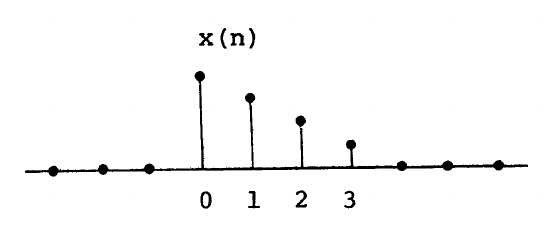
\includegraphics[width=0.5\linewidth]{img/img01}
			\caption{finite-length sequence $ x(n) $}
			\label{fig:img01}
		\end{figure}
		
		Jawaban: 
		\begin{figure}[H]
			\centering
			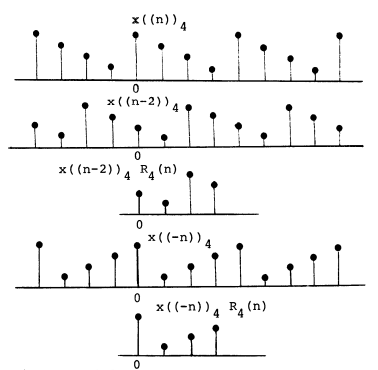
\includegraphics[width=0.5\linewidth]{img/img03}
			\caption{finite-length sequence $ x_1(n) $ dan $ x_2(n) $}
			\label{fig:img03}
		\end{figure}
		
		\item Gambar \ref{fig:img02} di bawah menunjukkan 2 finite length sequence. Gambarlah circular convolution 6 point-nya
		
		\begin{figure}[H]
			\centering
			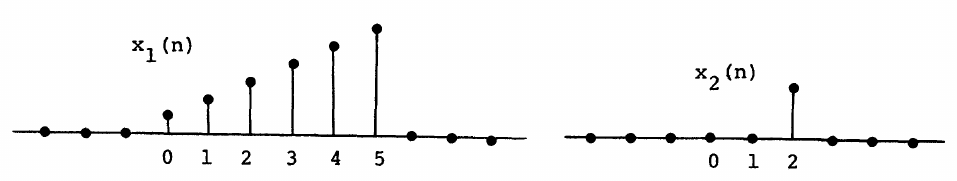
\includegraphics[width=0.7\linewidth]{img/img02}
			\caption{finite-length sequence $ x(n) $}
			\label{fig:img02}
		\end{figure}
		
		Jawaban:
		
		\begin{figure}[H]
			\centering
			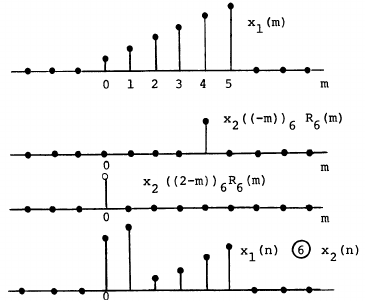
\includegraphics[width=0.5\linewidth]{img/img04}
			\caption{hasil circular convolution 6 point antara $ x_1(n) $ dengan $ x_2(n) $}
			\label{fig:img04}
		\end{figure}
	\end{enumerate}
\end{document}